\documentclass[11pt]{article}

\usepackage[margin=1in]{geometry}
\usepackage{fontspec}
\usepackage{microtype}
\usepackage{amsmath,amssymb}
\usepackage{booktabs}
\usepackage{graphicx}
\usepackage{subcaption}
\usepackage{siunitx}
\usepackage{xcolor}
\usepackage{enumitem}
\usepackage{fancyvrb}
\usepackage[numbers,sort&compress]{natbib}
\usepackage[colorlinks=true,linkcolor=blue!45!black,citecolor=blue!45!black,urlcolor=blue!45!black]{hyperref}
\usepackage[nameinlink,capitalise,noabbrev]{cleveref}

\graphicspath{
  {figures/}
  {../result/summary_plots/}
  {../result/eda/}
  {../result/evaluation/resnet18_unfrozen_from_frozen_lr1e-4_128_e8/test_20260508_104533/}
  {../result/gradcam/resnet18_unfrozen_from_frozen_lr1e-4_128_e8/gradcam_20260508_104648/}
}

\sisetup{
  round-mode=places,
  round-precision=4,
  table-number-alignment=center
}

\title{Transfer Learning and Error Analysis for Binary Food Image Classification}
\author{Xutong Dong \and Zhaoning Liang \and Yirong Li \and Jiaxu Zhang}
\date{May 2026}

\newcommand{\Healthy}{\textsc{healthy}}
\newcommand{\Unhealthy}{\textsc{unhealthy}}

\begin{document}

\maketitle

\begin{abstract}
This paper summarizes a reproducible binary food image classification study that distinguishes \Healthy{} and \Unhealthy{} food images. The project compares a small convolutional neural network trained from scratch, an ImageNet-pretrained ResNet18 with a frozen backbone, fully fine-tuned ResNet18 variants, and a supervised contrastive pretraining branch. On a balanced held-out test set of 522 images, the best observed model is a ResNet18 initialized from a frozen-transfer checkpoint and fully fine-tuned with learning rate \(10^{-4}\), achieving \(0.9617\) accuracy, \(0.9617\) macro F1, and \(0.9944\) ROC AUC. A focused ablation indicates that adapting high-level ResNet features accounts for most of the improvement over a frozen backbone, while full-backbone fine-tuning at the largest tested learning rate performs best. Error analysis shows 20 residual test errors, split evenly across the two classes.
\end{abstract}

\section{Introduction}

Image-based food classification is a practical visual recognition problem in which object appearance, plating context, and class definitions can all introduce ambiguity. This project studies a binary version of the task: each image is assigned to either \Healthy{} or \Unhealthy{}. The goal is not to claim nutritional ground truth beyond the dataset labels, but to evaluate whether modern transfer learning methods can produce reliable predictions under a fixed train/validation/test protocol.

The project is organized as an incremental empirical study. It begins with exploratory data analysis and a compact convolutional neural network (CNN) baseline, then compares the baseline with ImageNet-pretrained ResNet18 transfer learning. The transfer model is evaluated both with a frozen feature extractor and with subsequent fine-tuning. A supervised contrastive learning branch is also included to test whether label-aware representation learning improves the small CNN encoder. Finally, the strongest ResNet18 configuration is examined through a focused ablation and an error analysis of held-out test predictions. The repository \texttt{README.md} documents the pipeline commands, generated artifacts, and reproduction workflow used to produce the summaries cited in this paper \citep{projectreadme}. Team collaboration and code versioning were managed through GitHub at \url{https://github.com/JiaxuZhang-03/I242BProject} \citep{projectrepo}.

The current dataset contains 5,222 images with balanced class counts in all splits: 4,178 training images, 522 validation images, and 522 test images. Because the two classes are balanced, accuracy, macro F1, and weighted F1 are directly comparable for the main evaluation. The best model observed in the generated results is a fully fine-tuned ResNet18 initialized from a frozen-transfer checkpoint. It reaches \(0.9617\) test accuracy and \(0.9944\) ROC AUC, improving substantially over both the simple CNN baseline and the frozen-backbone transfer model.

\Cref{fig:dataset-overview} shows the split-level class counts and a sample grid generated during exploratory analysis.

\begin{figure}[t]
  \centering
  \begin{subfigure}[t]{0.43\linewidth}
    \centering
    \includegraphics[width=\linewidth]{dataset_counts.png}
    \caption{Class counts by split.}
  \end{subfigure}
  \hfill
  \begin{subfigure}[t]{0.53\linewidth}
    \centering
    \includegraphics[width=\linewidth]{sample_grid_train.png}
    \caption{Training-set examples.}
  \end{subfigure}
  \caption{Exploratory data analysis artifacts from \texttt{result/eda}. The dataset is balanced across \Healthy{} and \Unhealthy{} labels in the training, validation, and test splits.}
  \label{fig:dataset-overview}
\end{figure}

\section{Related Work}

Convolutional neural networks remain a standard architecture family for image recognition because they combine local receptive fields with hierarchical feature learning. Residual networks improve optimization by introducing skip connections, which allow deeper CNNs to learn residual mappings rather than entirely new transformations at each layer \citep{he2016deep}. In this project, ResNet18 is used as a computationally modest transfer-learning backbone.

Transfer learning is especially useful when task-specific datasets are smaller than the datasets used to train general-purpose visual encoders. ImageNet pretraining provides features learned from a large and diverse image collection \citep{deng2009imagenet}. The project evaluates two common transfer-learning regimes: training only a new classification head while freezing the backbone, and unfreezing part or all of the pretrained backbone for task-specific fine-tuning.

The supervised contrastive learning branch follows the idea that examples sharing a label should be close in representation space, while examples from different labels should be separated \citep{khosla2020supervised}. This objective is tested as an alternative representation-learning strategy for the simple CNN encoder. The resulting encoder is then fine-tuned for binary classification.

For interpretability, the project generates Grad-CAM visualizations \citep{selvaraju2017gradcam}. These maps are not treated as causal explanations, but they provide a qualitative check on which image regions influence the selected ResNet18 model. The implementation uses PyTorch for training and evaluation \citep{paszke2019pytorch}, AdamW for optimization \citep{loshchilov2019decoupled}, and standard image augmentations consistent with modern CNN training practice \citep{szegedy2016rethinking}.

\section{Method}

\subsection{Problem Setup}

Let \(\mathcal{D}=\{(x_i,y_i)\}_{i=1}^{n}\) denote the image dataset, where \(x_i\) is an RGB food image and \(y_i \in \{0,1\}\) indicates the class label. The model produces logits \(z_i=f_\theta(x_i)\in\mathbb{R}^{2}\), and class probabilities are computed by
\begin{equation}
  p_\theta(y=c\mid x_i)=\frac{\exp(z_{ic})}{\sum_{k=1}^{2}\exp(z_{ik})}.
\end{equation}
Classifier training minimizes the regularized empirical risk
\begin{equation}
  \min_{\theta}\;
  \frac{1}{n}\sum_{i=1}^{n}
  L_{\mathrm{ce}}\!\left(f_\theta(x_i),y_i\right)
  +\lambda\lVert\theta_{\mathrm{train}}\rVert_2^2,
\end{equation}
where \(L_{\mathrm{ce}}\) is cross-entropy and \(\theta_{\mathrm{train}}\) denotes the parameters updated in a given experiment. In implementation, the \(L_2\)-style penalty is applied through AdamW weight decay. Dropout in the classifier head, data augmentation, cosine learning-rate decay, and validation-based early stopping provide additional regularization.

\subsection{Data Processing}

The project uses an ImageFolder-style directory layout with separate \texttt{train}, \texttt{val}, and \texttt{test} folders. Images are resized to \(128\times128\) pixels for the current reported experiments. Training uses random resized crops, horizontal flips, and color jitter. Validation and test evaluation use deterministic resizing followed by center cropping. All images are normalized using ImageNet channel statistics, which is appropriate for the pretrained ResNet18 branch.

\begin{table}[t]
  \centering
  \caption{Dataset split sizes from \texttt{result/eda/dataset\_counts.csv}.}
  \label{tab:dataset}
  \begin{tabular}{lrrr}
    \toprule
    Split & Healthy & Unhealthy & Total \\
    \midrule
    Train & 2089 & 2089 & 4178 \\
    Validation & 261 & 261 & 522 \\
    Test & 261 & 261 & 522 \\
    \bottomrule
  \end{tabular}
\end{table}

\subsection{Models}

The simple CNN baseline uses four convolutional blocks with batch normalization, ReLU activations, and max pooling in the first three blocks. Adaptive average pooling converts the final feature map into a 256-dimensional feature vector. A dropout layer and linear classifier map this feature vector to two logits.

The transfer-learning models use a ResNet18 backbone. In the frozen-backbone configuration, ImageNet weights initialize the encoder and only the final binary classification head is trained. In the fine-tuning configurations, the model is initialized from the frozen-transfer checkpoint and then trained with either only ResNet \texttt{layer4} unfrozen or the full backbone unfrozen. The ablation varies the trainable scope and learning rate.

\subsection{Advanced Extension: Supervised Contrastive Branch}

The advanced methodological extension in this project is supervised contrastive pretraining, which is evaluated as a representation-learning alternative to direct cross-entropy training. For this branch, each training image is transformed into two augmented views. Let \(u_i\) and \(v_i\) denote normalized projected embeddings. The supervised contrastive loss encourages embeddings with the same label to have high cosine similarity and embeddings with different labels to have lower similarity:
\begin{equation}
  \mathcal{L}_{\mathrm{supcon}}
  =
  \sum_{i}
  \frac{-1}{|P(i)|}
  \sum_{p\in P(i)}
  \log
  \frac{\exp(\operatorname{sim}(u_i,v_p)/\tau)}
       {\sum_{a\neq i}\exp(\operatorname{sim}(u_i,v_a)/\tau)},
\end{equation}
where \(P(i)\) is the set of same-label positives for anchor \(i\), \(\operatorname{sim}(\cdot,\cdot)\) is cosine similarity after normalization, and \(\tau=0.07\) in the current implementation. The pretrained encoder is then reused in a classifier and fine-tuned with cross-entropy.

\subsection{Evaluation}

Each classifier is evaluated on the held-out test set. The generated summaries report accuracy, macro F1, weighted F1, and ROC AUC. For binary classification, the confusion matrix is
\begin{equation}
  C_{ab}=\left|\{i:y_i=a,\hat{y}_i=b\}\right|,
\end{equation}
where \(a\) is the true class and \(b\) is the predicted class. Error analysis additionally records misclassified samples, predicted-class confidence, class-specific error rates, and high-confidence errors.

\section{Experiments}

\subsection{Training Protocol}

All reported model runs use \(128\times128\) inputs and the balanced train/validation/test split in \cref{tab:dataset}. Classifiers are optimized with AdamW and cosine learning-rate scheduling. The baseline simple CNN, frozen ResNet18, and SupCon fine-tuned classifier are trained for five epochs in the current summary. ResNet18 fine-tuning runs for up to eight epochs, with early stopping available in the training script.

\begin{table}[t]
  \centering
  \caption{Held-out test results from \texttt{result/experiment\_summary.csv}.}
  \label{tab:main-results}
  \begin{tabular}{lS[table-format=1.4]S[table-format=1.4]S[table-format=1.4]S[table-format=1.4]}
    \toprule
    Experiment & {Best val. acc.} & {Test acc.} & {Macro F1} & {ROC AUC} \\
    \midrule
    ResNet18 full fine-tune, LR \(10^{-4}\) & 0.9655 & 0.9617 & 0.9617 & 0.9944 \\
    ResNet18 layer4 fine-tune, LR \(3\times10^{-5}\) & 0.9540 & 0.9406 & 0.9406 & 0.9850 \\
    ResNet18 full fine-tune, LR \(3\times10^{-5}\) & 0.9598 & 0.9406 & 0.9406 & 0.9845 \\
    ResNet18 full fine-tune, LR \(10^{-5}\) & 0.9406 & 0.9310 & 0.9310 & 0.9781 \\
    ResNet18 frozen backbone & 0.8563 & 0.8697 & 0.8697 & 0.9344 \\
    Simple CNN + SupCon fine-tune & 0.8084 & 0.8046 & 0.8033 & 0.8813 \\
    Simple CNN baseline & 0.7989 & 0.8027 & 0.8027 & 0.8869 \\
    \bottomrule
  \end{tabular}
\end{table}

\Cref{tab:main-results} shows that ImageNet transfer improves substantially over the simple CNN baseline, and that full ResNet18 fine-tuning gives the strongest result. The best model improves test accuracy from \(0.8697\) for the frozen-backbone ResNet18 to \(0.9617\), an absolute gain of \(0.0920\). It also improves ROC AUC from \(0.9344\) to \(0.9944\).

\begin{figure}[t]
  \centering
  \begin{subfigure}[t]{0.48\linewidth}
    \centering
    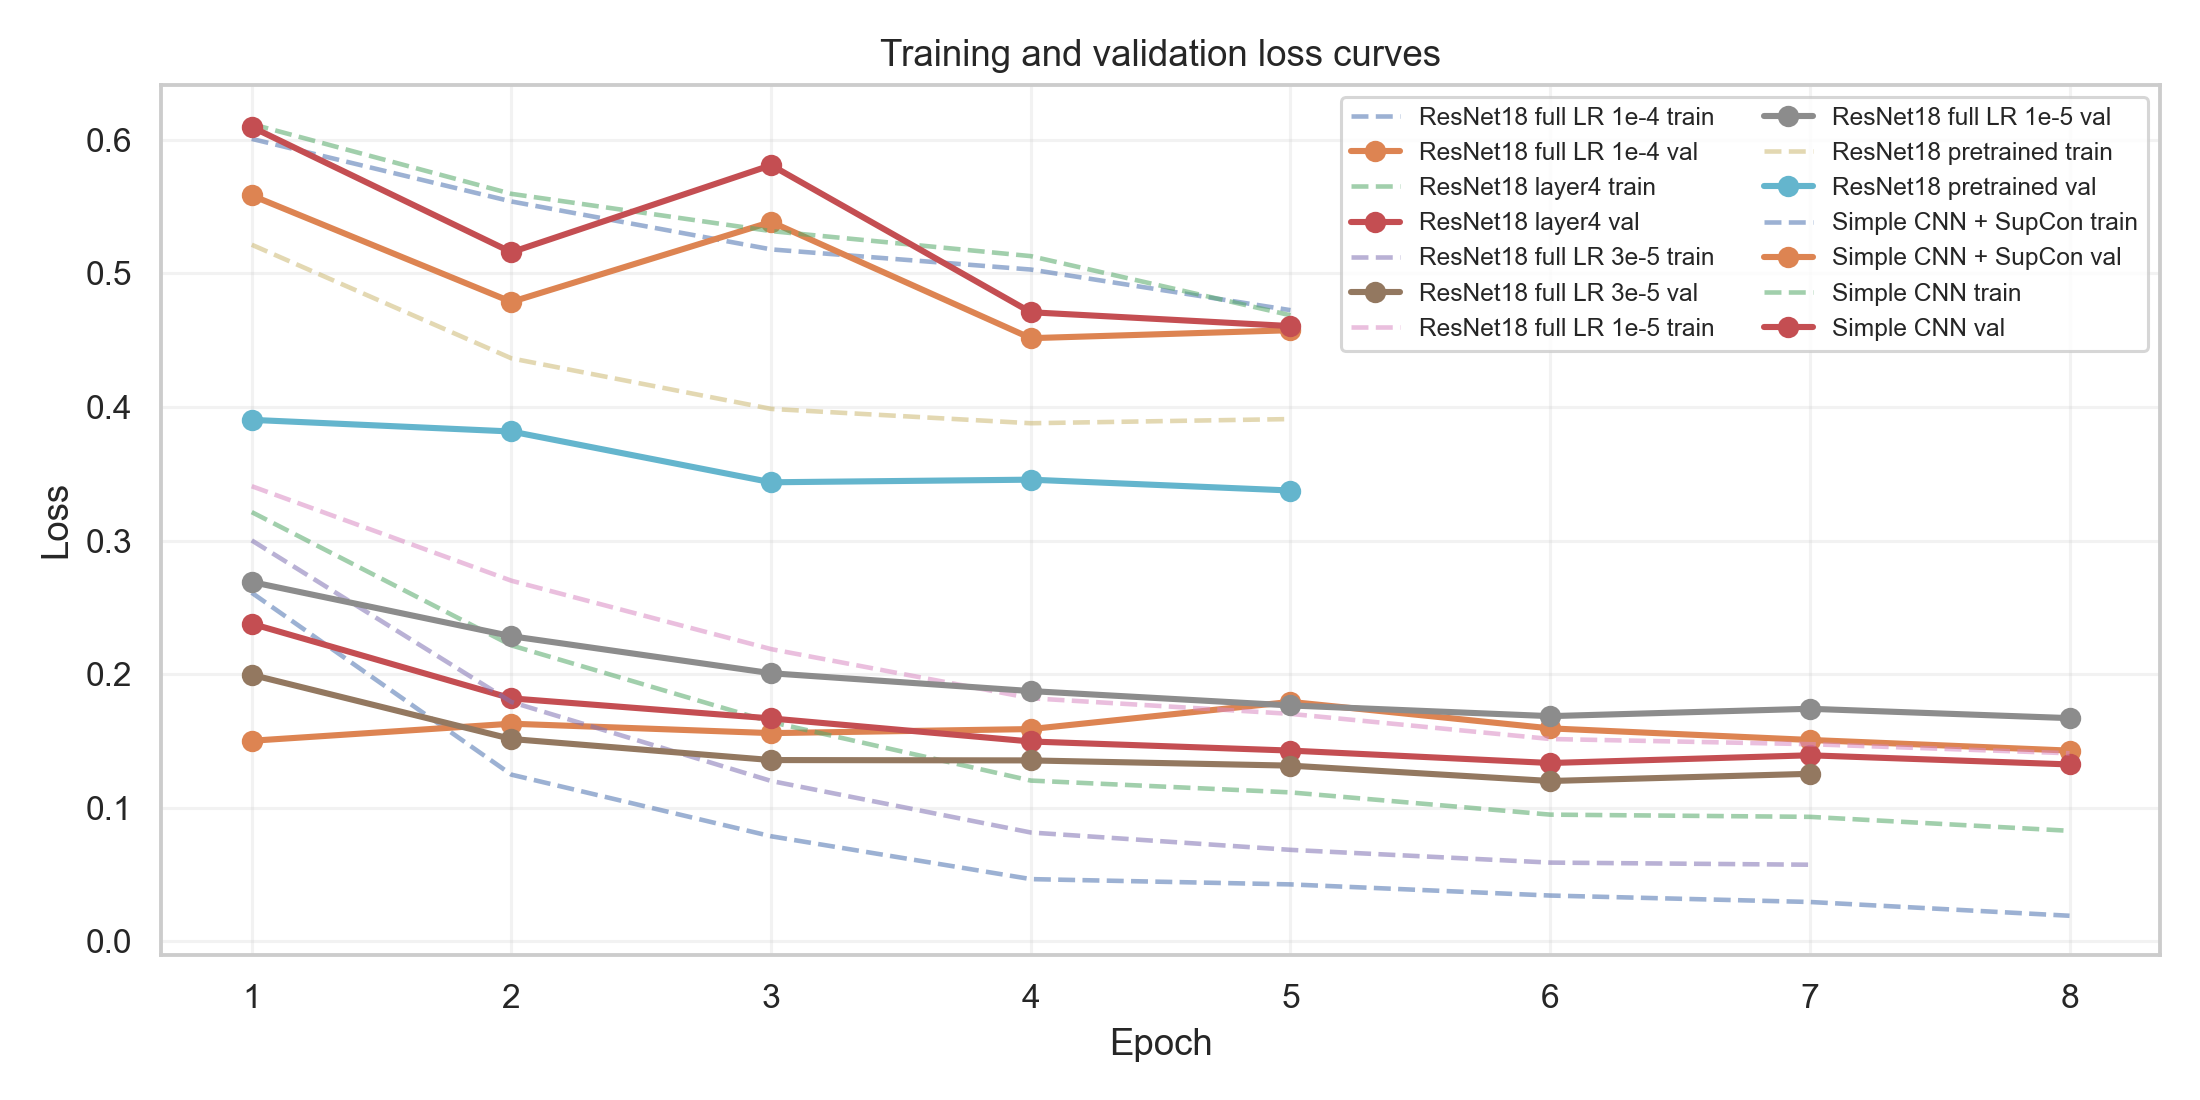
\includegraphics[width=\linewidth]{training_loss_curves.png}
    \caption{Training and validation loss.}
  \end{subfigure}
  \hfill
  \begin{subfigure}[t]{0.48\linewidth}
    \centering
    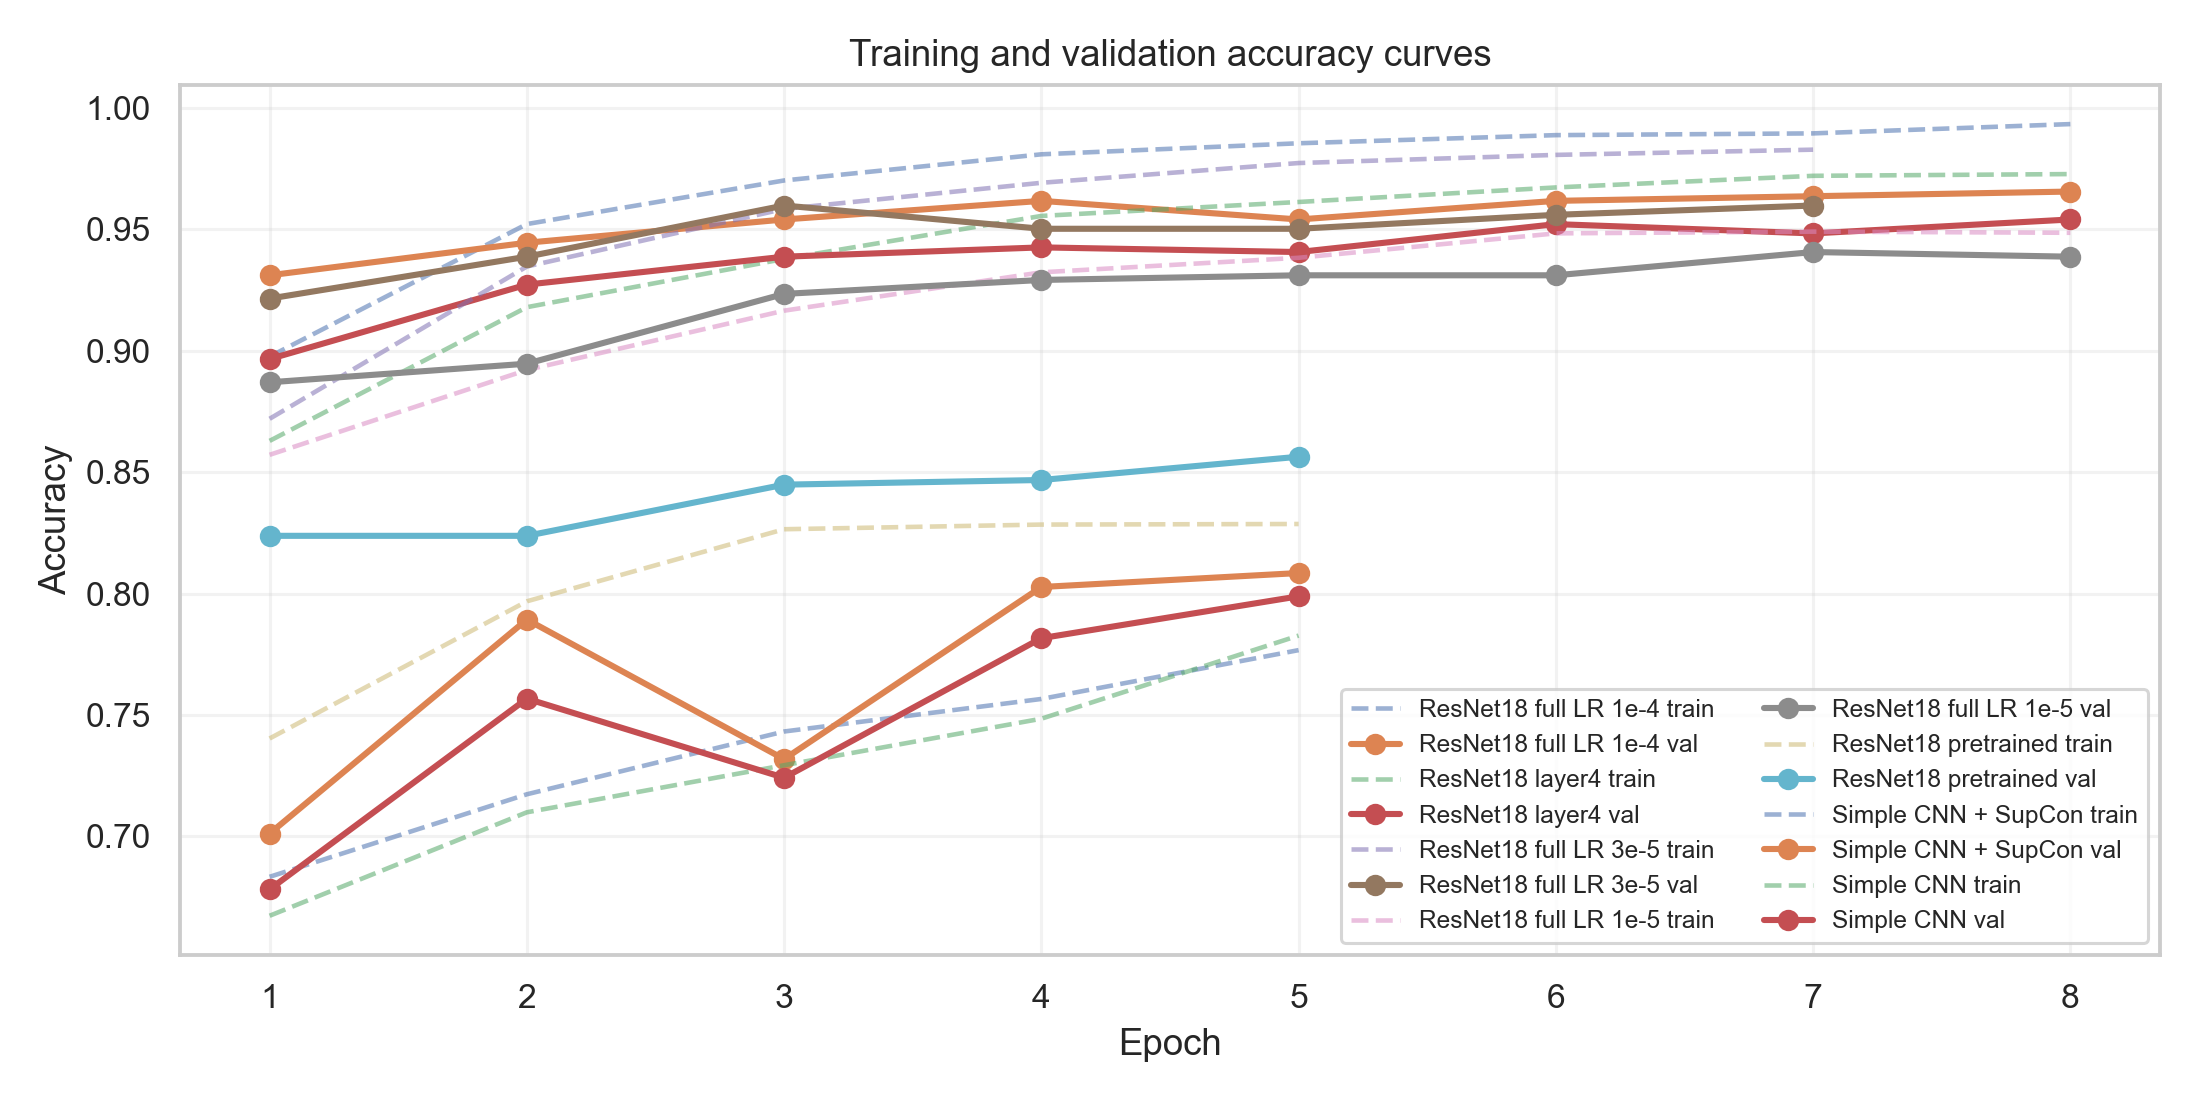
\includegraphics[width=\linewidth]{training_accuracy_curves.png}
    \caption{Training and validation accuracy.}
  \end{subfigure}
  \caption{Optimization diagnostics generated from the saved history files.}
  \label{fig:training-diagnostics}
\end{figure}

\Cref{fig:training-diagnostics} provides the main bias--variance diagnostic. The simple CNN and SupCon-initialized simple CNN remain below the ResNet18 variants, suggesting that the compact encoder underfits the task relative to the transferred residual backbone. The best full fine-tuned ResNet18 reaches high training accuracy while validation accuracy continues to improve through the final epoch, so the saved curves do not show severe validation collapse. The gap between training and validation loss nevertheless grows during fine-tuning, which indicates that regularization and validation monitoring remain important for this dataset.

\begin{figure}[t]
  \centering
  \begin{subfigure}[t]{0.48\linewidth}
    \centering
    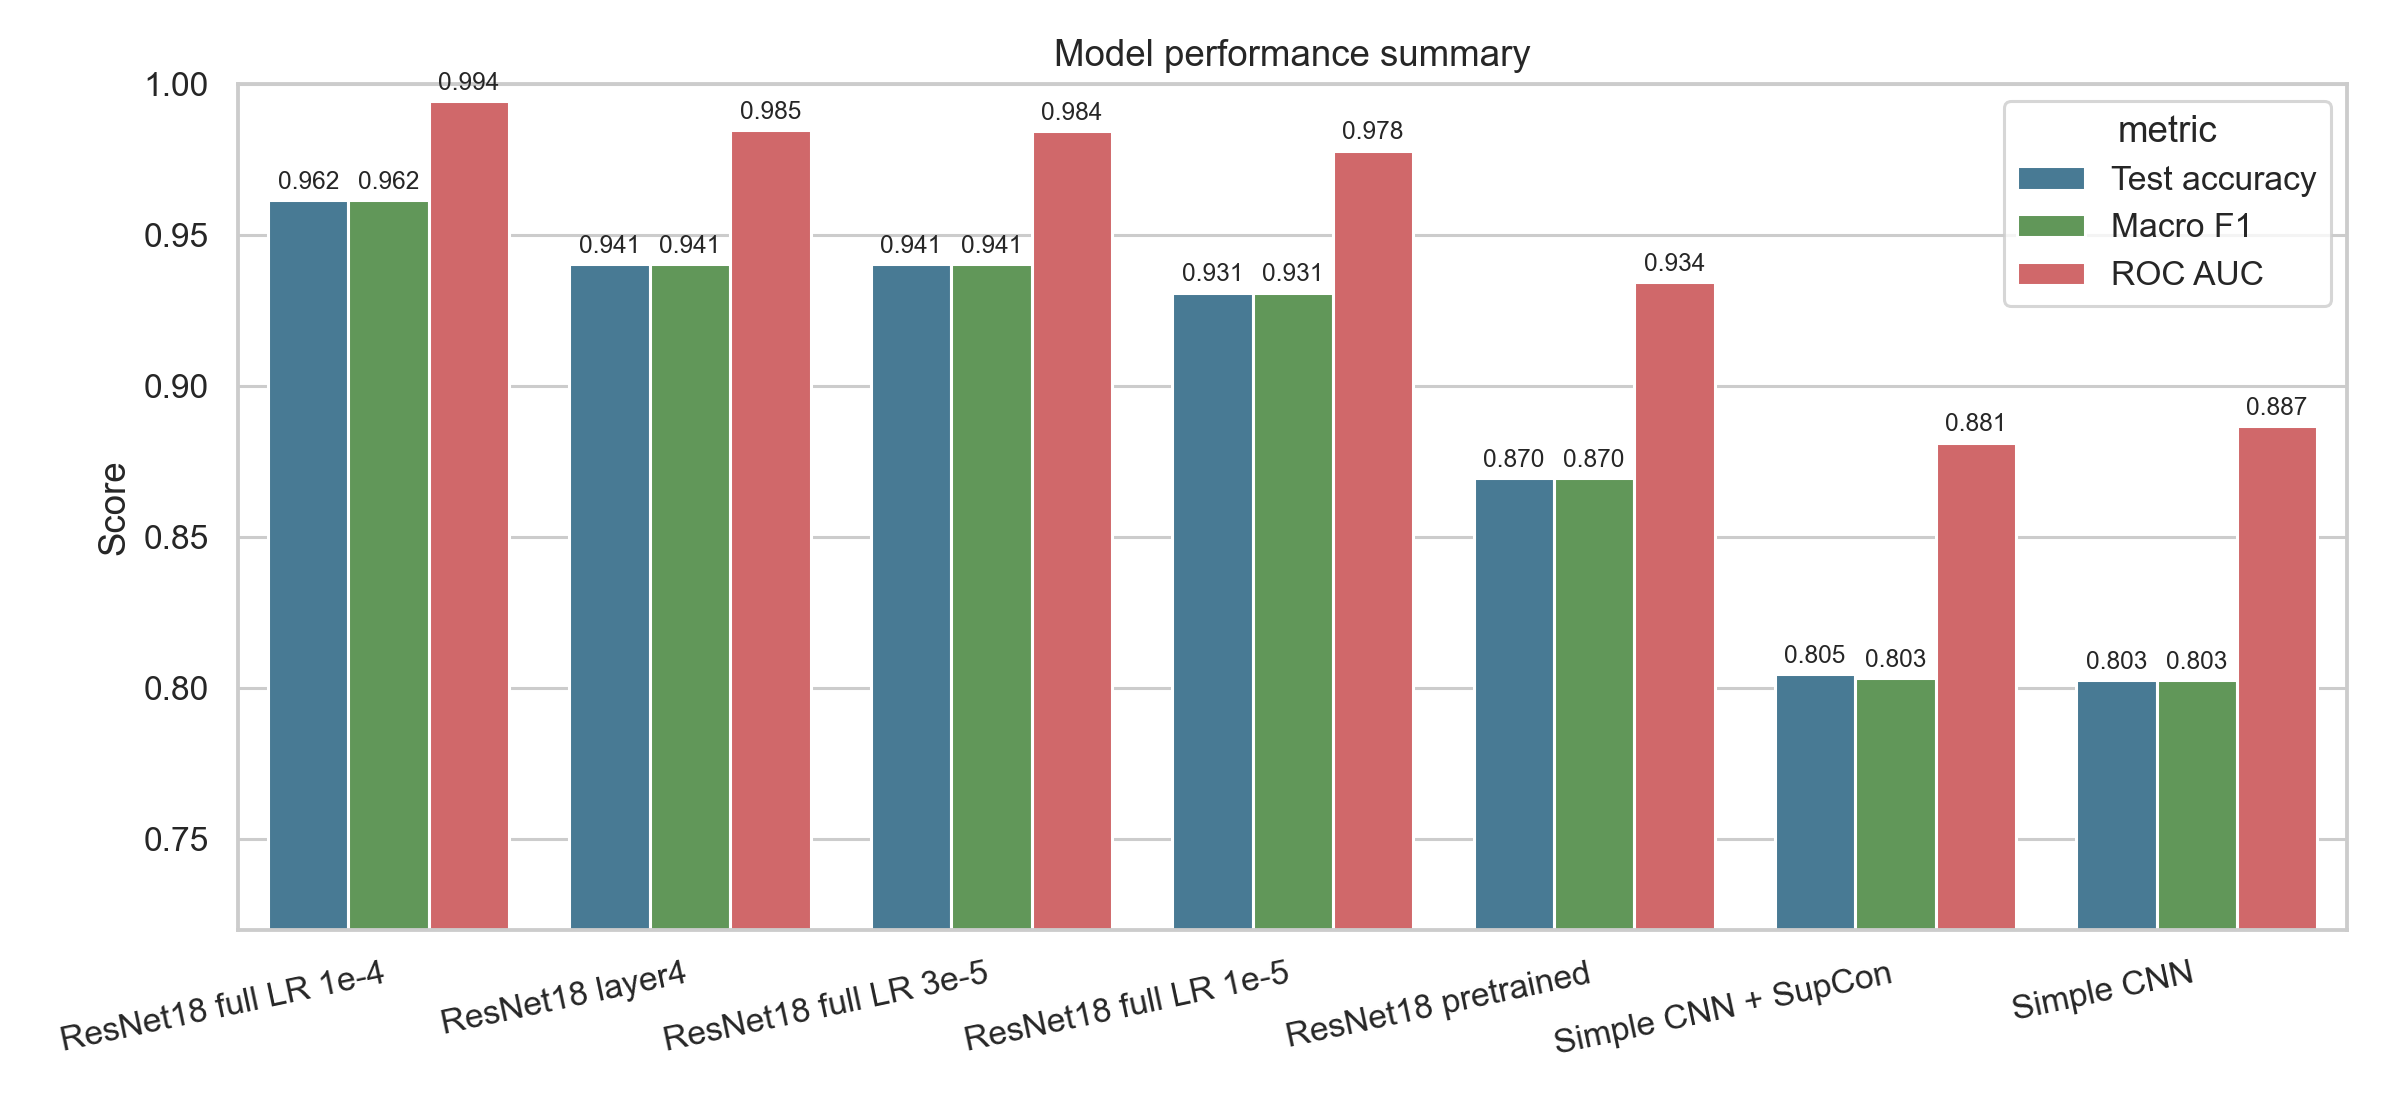
\includegraphics[width=\linewidth]{model_metric_comparison.png}
    \caption{Model metric comparison.}
  \end{subfigure}
  \hfill
  \begin{subfigure}[t]{0.48\linewidth}
    \centering
    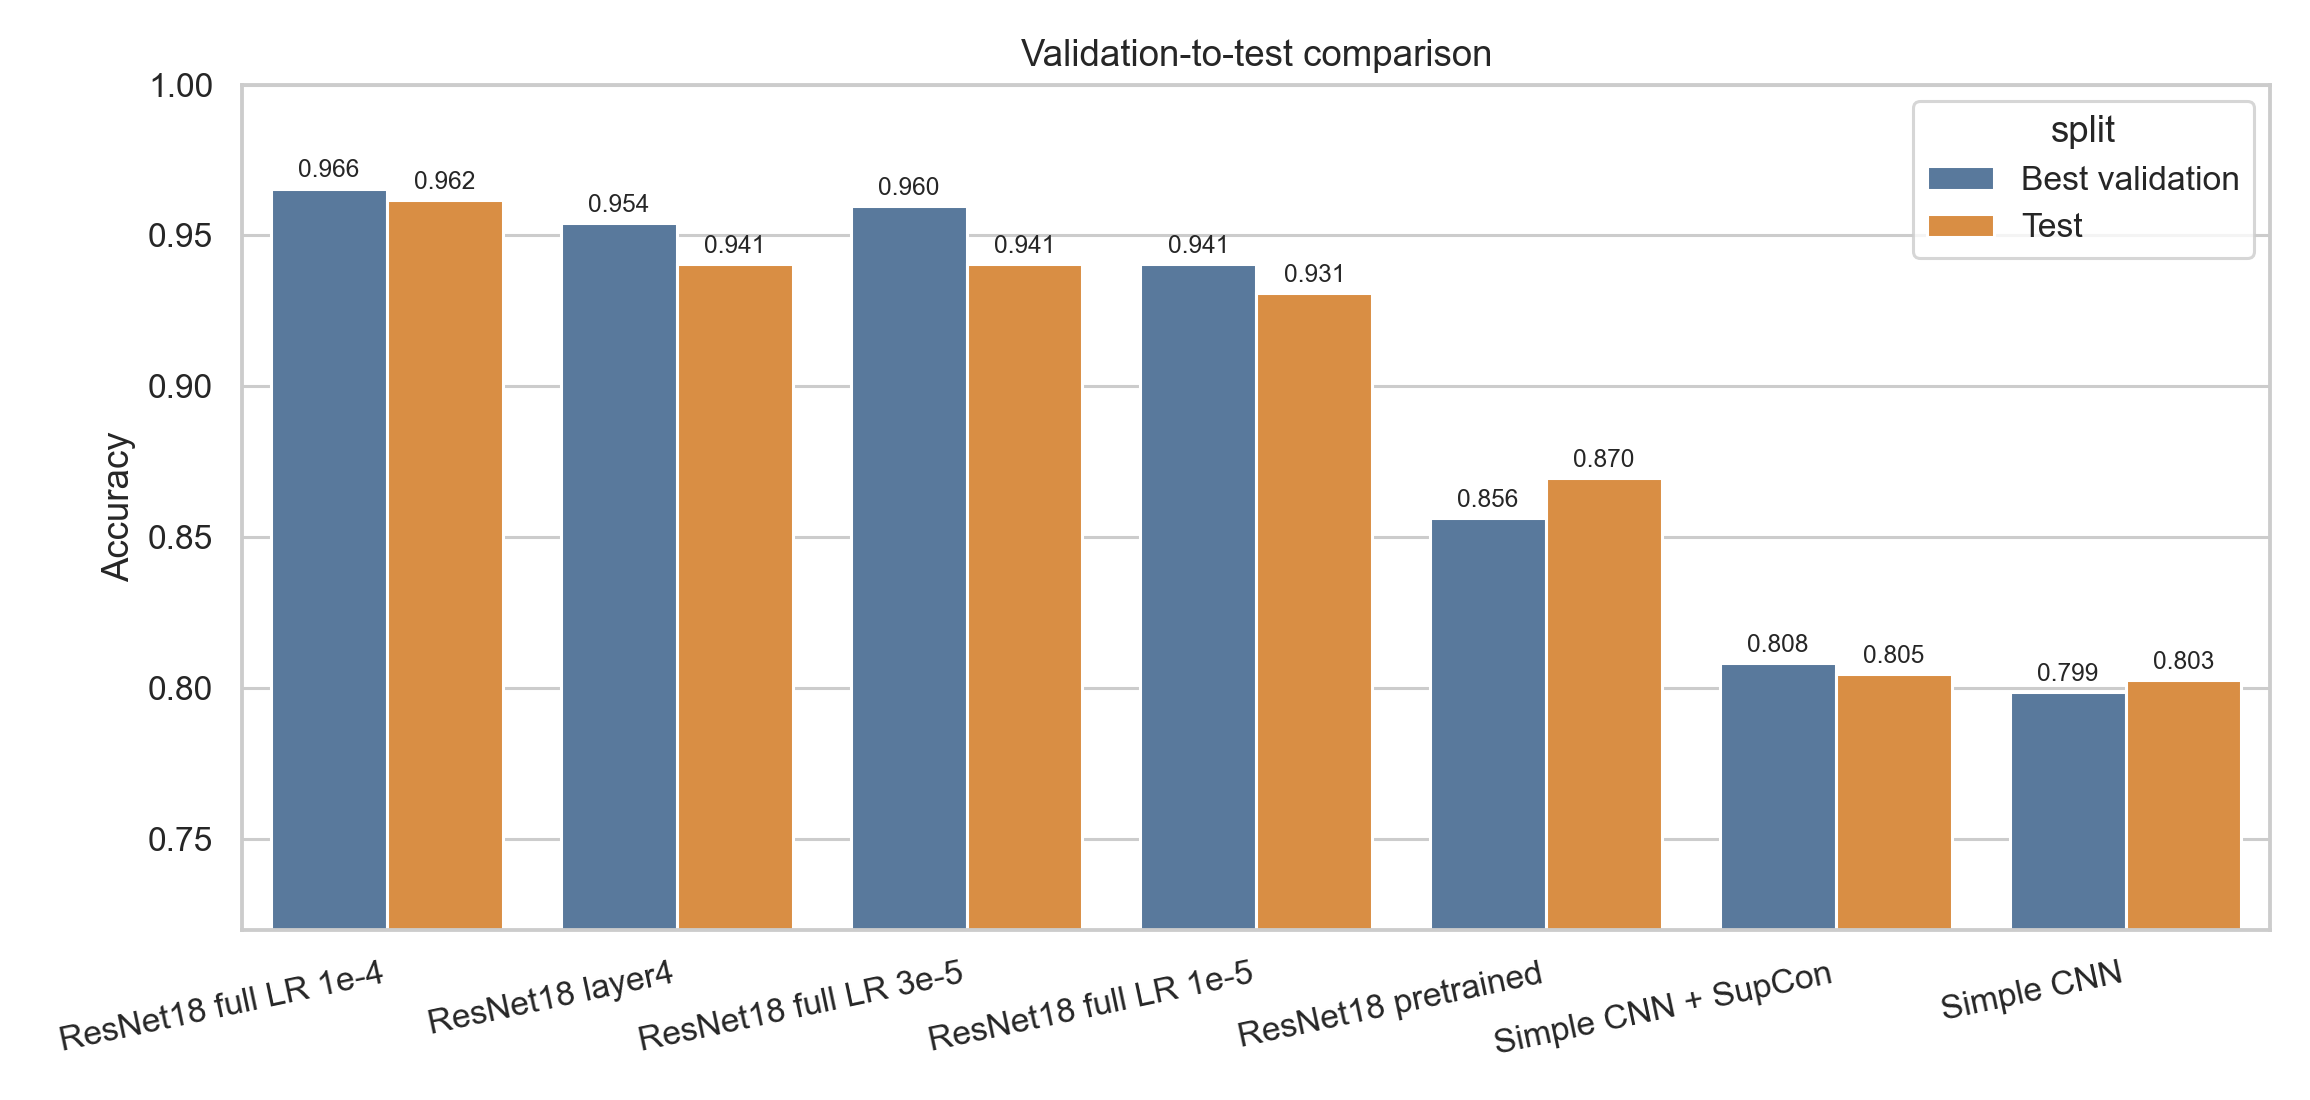
\includegraphics[width=\linewidth]{validation_vs_test_accuracy.png}
    \caption{Validation and test accuracy.}
  \end{subfigure}
  \caption{Summary plots generated from the experiment outputs in \texttt{result/summary\_plots}.}
  \label{fig:model-summary}
\end{figure}

\subsection{Ablation}

The ResNet18 ablation separates the effects of initialization, trainable scope, and learning rate. Training only the classifier head provides a useful transfer baseline but reaches only \(0.8697\) test accuracy. Unfreezing ResNet \texttt{layer4} raises accuracy to \(0.9406\), indicating that high-level feature adaptation explains much of the gain. Full-backbone fine-tuning is sensitive to the learning rate: \(10^{-5}\) under-adapts in the current run, \(3\times10^{-5}\) matches the layer4 setting, and \(10^{-4}\) achieves the best test accuracy.

\begin{table}[t]
  \centering
  \caption{Focused ResNet18 fine-tuning ablation from \texttt{result/ablation\_summary.csv}.}
  \label{tab:ablation}
  \begin{tabular}{llS[table-format=1.5]S[table-format=1.4]S[table-format=1.4]r}
    \toprule
    Setting & Trainable scope & {LR} & {Test acc.} & {ROC AUC} & {Trainable params} \\
    \midrule
    Frozen head & classifier head & 0.001 & 0.8697 & 0.9344 & 1026 \\
    Layer4 fine-tune & classifier + layer4 & 0.00003 & 0.9406 & 0.9850 & 8394754 \\
    Full fine-tune & full backbone & 0.00001 & 0.9310 & 0.9781 & 11177538 \\
    Full fine-tune & full backbone & 0.00003 & 0.9406 & 0.9845 & 11177538 \\
    Full fine-tune & full backbone & 0.0001 & 0.9617 & 0.9944 & 11177538 \\
    \bottomrule
  \end{tabular}
\end{table}

\begin{figure}[t]
  \centering
  \begin{subfigure}[t]{0.48\linewidth}
    \centering
    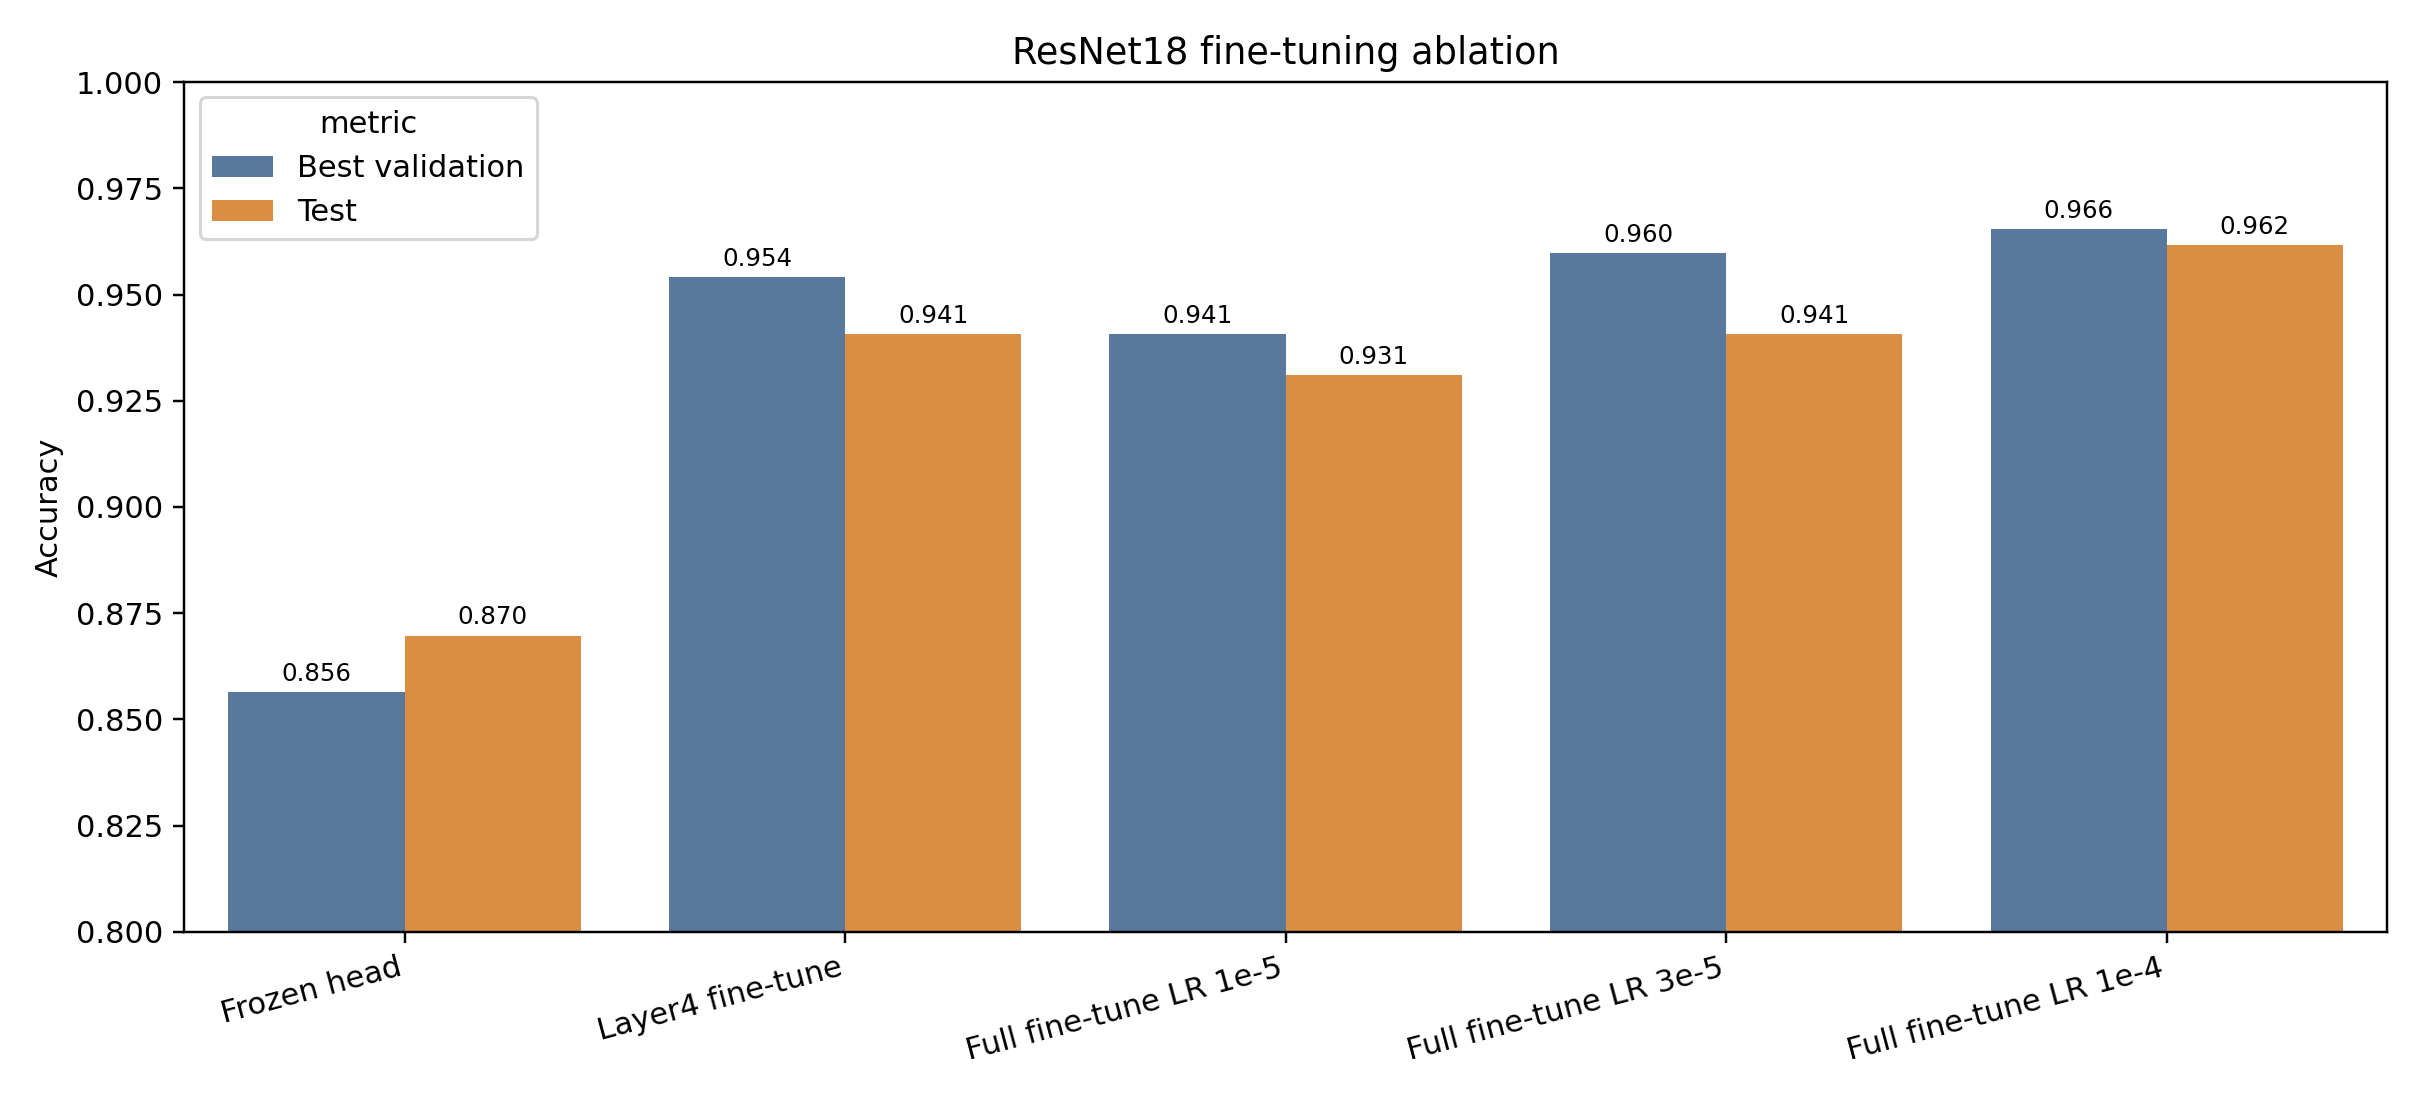
\includegraphics[width=\linewidth]{resnet18_ablation_accuracy.png}
    \caption{Ablation accuracy.}
  \end{subfigure}
  \hfill
  \begin{subfigure}[t]{0.48\linewidth}
    \centering
    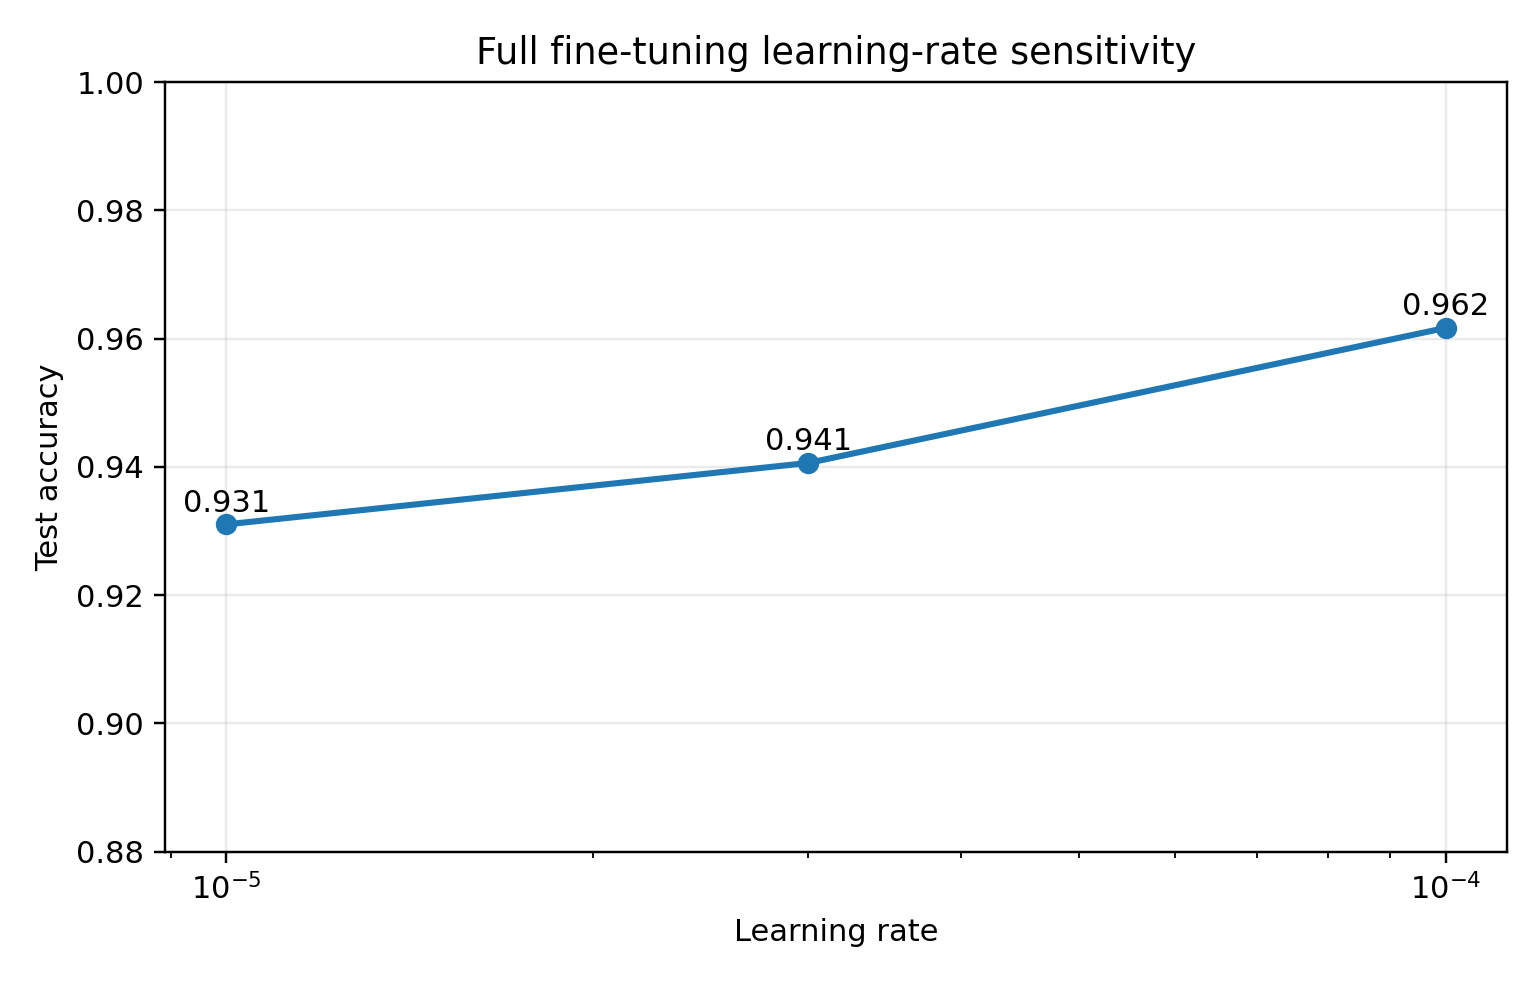
\includegraphics[width=\linewidth]{resnet18_ablation_lr_sensitivity.png}
    \caption{Learning-rate sensitivity.}
  \end{subfigure}
  \caption{ResNet18 ablation plots generated from \texttt{result/ablation\_summary.csv}.}
  \label{fig:ablation}
\end{figure}

\subsection{Error Analysis}

The best model makes 20 errors on 522 test images. Errors are balanced across classes: 10 \Healthy{} images are predicted as \Unhealthy{}, and 10 \Unhealthy{} images are predicted as \Healthy{}. The resulting confusion matrix is shown in \cref{tab:confusion}. The mean predicted-class confidence among errors is \(0.7843\), and 12 of the 20 errors have confidence at least \(0.80\). These high-confidence failures are useful targets for qualitative inspection because they are not simply low-confidence borderline predictions.

\begin{table}[t]
  \centering
  \caption{Confusion matrix for the best ResNet18 model on the test set.}
  \label{tab:confusion}
  \begin{tabular}{lrr}
    \toprule
    True class & Predicted healthy & Predicted unhealthy \\
    \midrule
    Healthy & 251 & 10 \\
    Unhealthy & 10 & 251 \\
    \bottomrule
  \end{tabular}
\end{table}

\begin{figure}[t]
  \centering
  \begin{subfigure}[t]{0.48\linewidth}
    \centering
    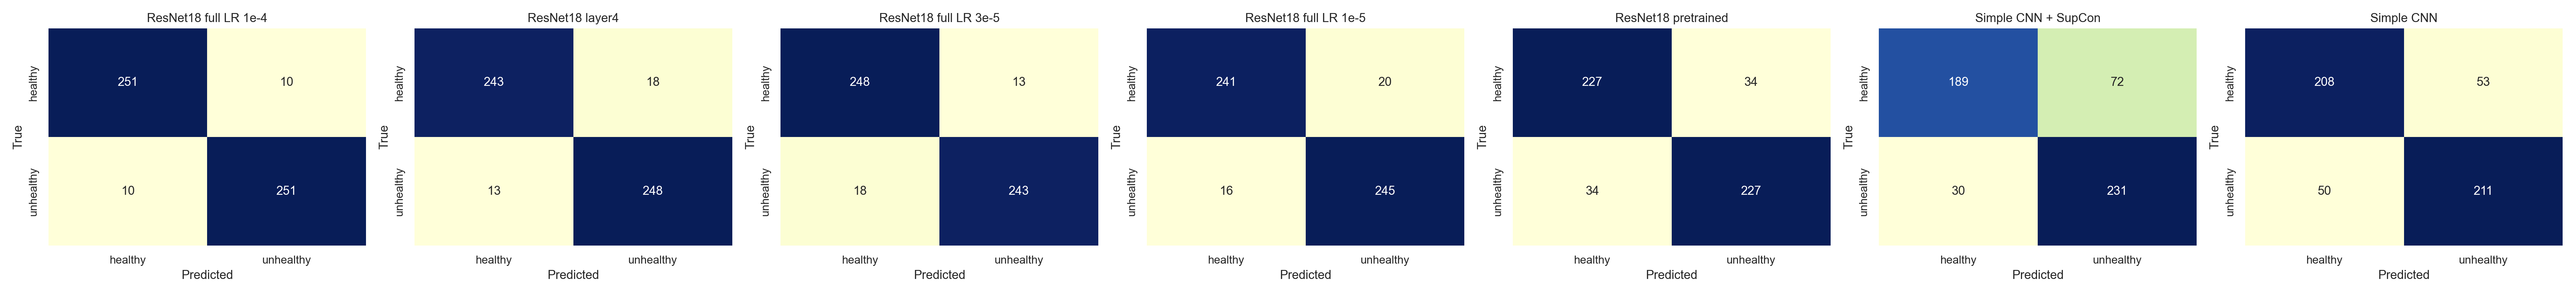
\includegraphics[width=\linewidth]{test_confusion_matrices.png}
    \caption{Test confusion matrices.}
  \end{subfigure}
  \hfill
  \begin{subfigure}[t]{0.48\linewidth}
    \centering
    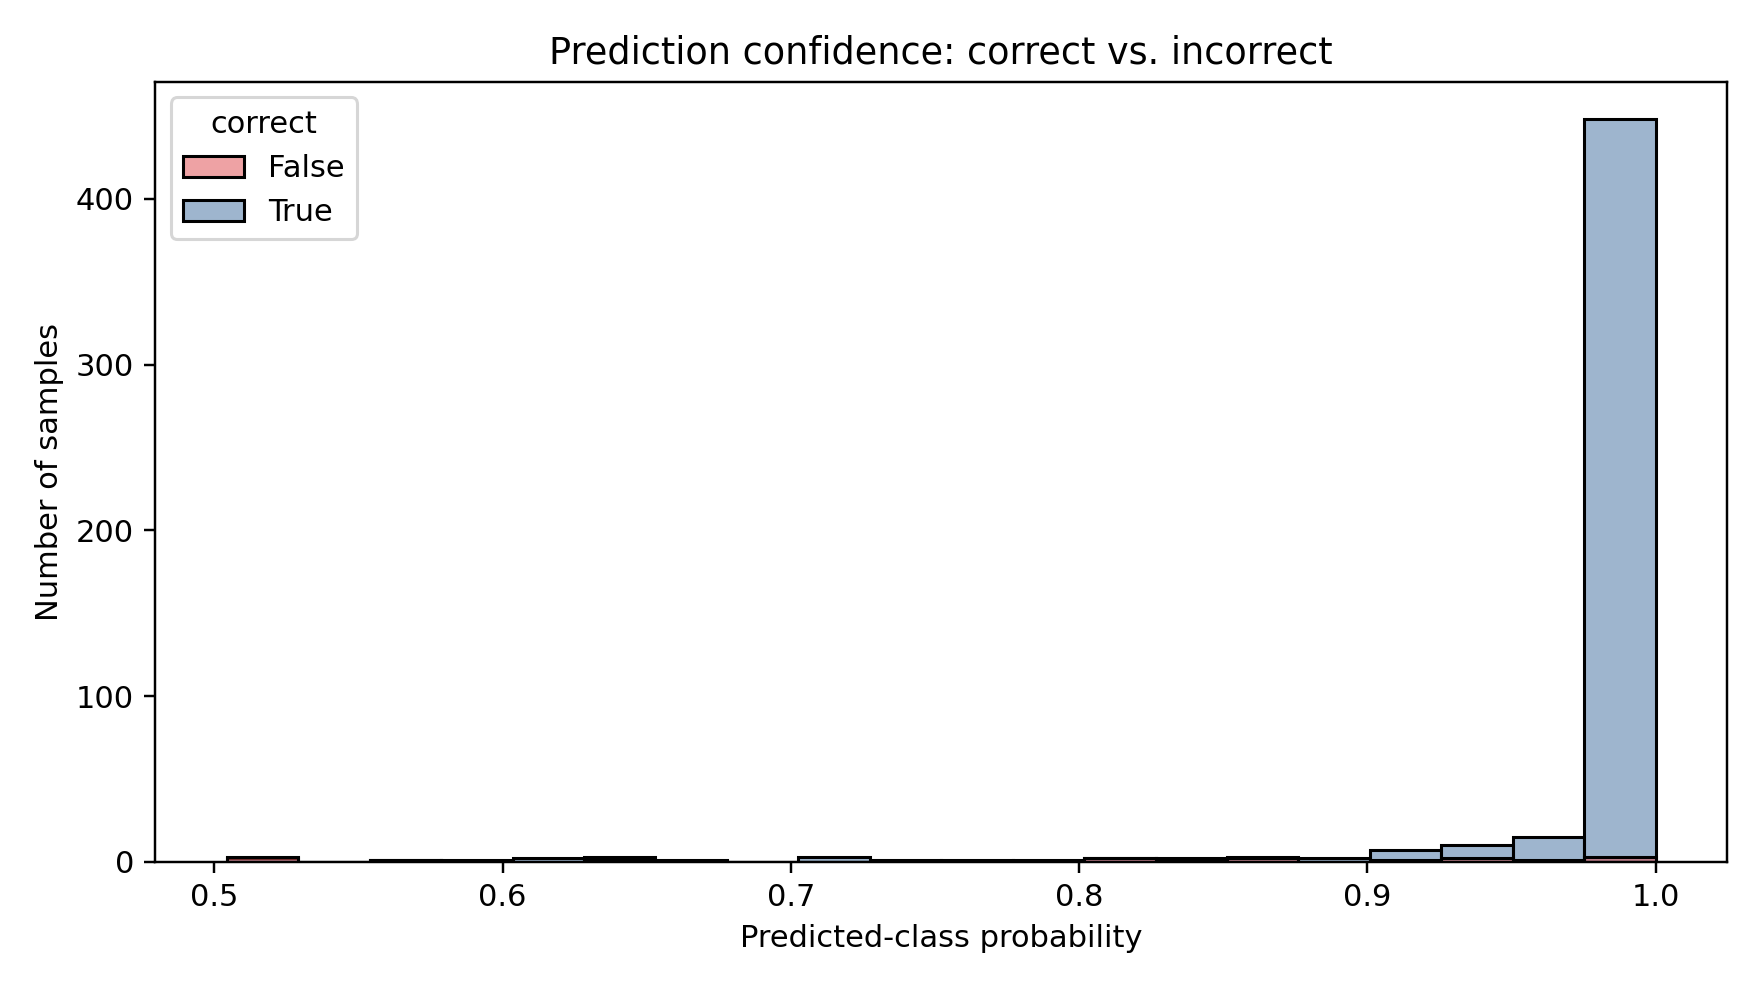
\includegraphics[width=\linewidth]{error_confidence_histogram.png}
    \caption{Confidence of residual errors.}
  \end{subfigure}
  \caption{Evaluation and error-analysis plots from \texttt{result/summary\_plots}.}
  \label{fig:error-analysis}
\end{figure}

\begin{figure}[t]
  \centering
  \includegraphics[width=0.8\linewidth]{009_img_51f7253d21_gradcam.png}
  \caption{Example Grad-CAM artifact for the selected ResNet18 model. Additional Grad-CAM images are stored under \texttt{result/gradcam}. This figure is qualitative and is not used as quantitative evidence.}
  \label{fig:gradcam}
\end{figure}

\subsection{Missing or Future Results}

The repository contains the main summaries, ablation outputs, error-analysis tables, and visual artifacts needed for the current report. Additional experiments, such as longer SupCon pretraining, larger backbones, confidence calibration, or cross-dataset validation, have not been run in the provided artifacts. For that reason, this report does not claim results for those extensions.

\section{Safety, Security, and Ethics}

The model should not be deployed as an authoritative nutrition or health advisor. The labels \Healthy{} and \Unhealthy{} simplify a complex nutritional judgment that depends on ingredients, portion size, preparation, culture, dietary constraints, and individual medical context. A visually plausible prediction can therefore be misleading even when the classifier is accurate on the held-out dataset.

At large scale, the main safety risk is over-reliance: users or organizations might treat the output as dietary guidance rather than a coarse visual categorization. The observed \(0.9617\) test accuracy still corresponds to 20 errors on 522 held-out images, including 12 high-confidence errors. A production system would need calibrated uncertainty, human review for high-impact uses, clearer label definitions, and evaluation on data collected from the intended deployment population.

There are also fairness and privacy concerns. Food appearance varies by cuisine, region, socioeconomic context, and image quality; a model trained on one dataset may perform worse on underrepresented foods or presentation styles. If user-uploaded meal images were collected, the system would need safeguards for consent, retention, access control, and removal of incidental personal information. For these reasons, the current project is best viewed as a controlled academic study and not as a ready-to-deploy health tool.

\section{Conclusion}

This project demonstrates that transfer learning is the dominant performance driver for the binary food image classification task studied here. A simple CNN trained from scratch reaches \(0.8027\) test accuracy, while a frozen ImageNet-pretrained ResNet18 improves to \(0.8697\). Fine-tuning the pretrained ResNet18 provides the largest gain, with the best current configuration reaching \(0.9617\) test accuracy and \(0.9944\) ROC AUC.

The ablation suggests that adapting high-level residual features is already sufficient to capture much of the improvement, but full-backbone fine-tuning with learning rate \(10^{-4}\) performs best among the tested settings. The final error analysis shows balanced residual errors across \Healthy{} and \Unhealthy{} classes, with several high-confidence mistakes that warrant qualitative review. Future work should avoid reporting speculative gains and instead extend the present pipeline with new generated summaries for longer training, alternative backbones, calibration analysis, or evaluation on an independently collected dataset.


\bibliographystyle{plainnat}
\bibliography{references}

\appendix
\section{Code and Reproducibility}

The project code is organized as executable scripts and reusable modules. The repository \texttt{README.md} documents the full workflow. The team used GitHub for code collaboration, version control, and project sharing: \url{https://github.com/JiaxuZhang-03/I242BProject}. An interactive Docker-deployed demo is available as a \href{https://huggingface.co/spaces/LittleOtterUD/INDENGInterface}{Hugging Face Spaces interface}.

\begin{itemize}[leftmargin=*]
  \item \texttt{src/train\_classifier.py}: classifier training, transfer learning, checkpoint initialization, and fine-tuning policies.
  \item \texttt{src/pretrain\_supcon.py}: supervised contrastive pretraining.
  \item \texttt{src/evaluate\_model.py}: held-out evaluation, metrics, predictions, ROC curves, and confusion matrices.
  \item \texttt{src/error\_analysis.py}: residual error summaries and high-confidence error analysis.
  \item \texttt{src/food\_project/models.py}: simple CNN, ResNet18 classifier wrappers, and SupCon projection head.
  \item \texttt{src/food\_project/data.py}: dataset discovery, transformations, dataloaders, and split summaries.
\end{itemize}

\noindent From the repository root, the complete pipeline can be reproduced with:

\begin{Verbatim}[fontsize=\small]
./download_data.sh
./setup_environment.sh
./run_full_pipeline.sh
./run_resnet_ablation.sh
\end{Verbatim}

\noindent Representative source excerpts are included below; the complete implementation is in the repository.

\subsection{Model Definition Excerpt}

\VerbatimInput[fontsize=\scriptsize,firstline=23,lastline=76]{../src/food_project/models.py}

\subsection{Fine-Tuning Policy Excerpt}

\VerbatimInput[fontsize=\scriptsize,firstline=53,lastline=85]{../src/train_classifier.py}


\end{document}
